% Options for packages loaded elsewhere
% Options for packages loaded elsewhere
\PassOptionsToPackage{unicode}{hyperref}
\PassOptionsToPackage{hyphens}{url}
%
\documentclass[
  ignorenonframetext,
]{beamer}
\newif\ifbibliography
\usepackage{pgfpages}
\setbeamertemplate{caption}[numbered]
\setbeamertemplate{caption label separator}{: }
\setbeamercolor{caption name}{fg=normal text.fg}
\beamertemplatenavigationsymbolsempty
% remove section numbering
\setbeamertemplate{part page}{
  \centering
  \begin{beamercolorbox}[sep=16pt,center]{part title}
    \usebeamerfont{part title}\insertpart\par
  \end{beamercolorbox}
}
\setbeamertemplate{section page}{
  \centering
  \begin{beamercolorbox}[sep=12pt,center]{section title}
    \usebeamerfont{section title}\insertsection\par
  \end{beamercolorbox}
}
\setbeamertemplate{subsection page}{
  \centering
  \begin{beamercolorbox}[sep=8pt,center]{subsection title}
    \usebeamerfont{subsection title}\insertsubsection\par
  \end{beamercolorbox}
}
% Prevent slide breaks in the middle of a paragraph
\widowpenalties 1 10000
\raggedbottom
\AtBeginPart{
  \frame{\partpage}
}
\AtBeginSection{
  \ifbibliography
  \else
    \frame{\sectionpage}
  \fi
}
\AtBeginSubsection{
  \frame{\subsectionpage}
}
\usepackage{iftex}
\ifPDFTeX
  \usepackage[T1]{fontenc}
  \usepackage[utf8]{inputenc}
  \usepackage{textcomp} % provide euro and other symbols
\else % if luatex or xetex
  \usepackage{unicode-math} % this also loads fontspec
  \defaultfontfeatures{Scale=MatchLowercase}
  \defaultfontfeatures[\rmfamily]{Ligatures=TeX,Scale=1}
\fi
\usepackage{lmodern}

\usetheme[]{sintef}
\ifPDFTeX\else
  % xetex/luatex font selection
\fi
% Use upquote if available, for straight quotes in verbatim environments
\IfFileExists{upquote.sty}{\usepackage{upquote}}{}
\IfFileExists{microtype.sty}{% use microtype if available
  \usepackage[]{microtype}
  \UseMicrotypeSet[protrusion]{basicmath} % disable protrusion for tt fonts
}{}
\makeatletter
\@ifundefined{KOMAClassName}{% if non-KOMA class
  \IfFileExists{parskip.sty}{%
    \usepackage{parskip}
  }{% else
    \setlength{\parindent}{0pt}
    \setlength{\parskip}{6pt plus 2pt minus 1pt}}
}{% if KOMA class
  \KOMAoptions{parskip=half}}
\makeatother


\usepackage{longtable,booktabs,array}
\usepackage{calc} % for calculating minipage widths
\usepackage{caption}
% Make caption package work with longtable
\makeatletter
\def\fnum@table{\tablename~\thetable}
\makeatother
\usepackage{graphicx}
\makeatletter
\newsavebox\pandoc@box
\newcommand*\pandocbounded[1]{% scales image to fit in text height/width
  \sbox\pandoc@box{#1}%
  \Gscale@div\@tempa{\textheight}{\dimexpr\ht\pandoc@box+\dp\pandoc@box\relax}%
  \Gscale@div\@tempb{\linewidth}{\wd\pandoc@box}%
  \ifdim\@tempb\p@<\@tempa\p@\let\@tempa\@tempb\fi% select the smaller of both
  \ifdim\@tempa\p@<\p@\scalebox{\@tempa}{\usebox\pandoc@box}%
  \else\usebox{\pandoc@box}%
  \fi%
}
% Set default figure placement to htbp
\def\fps@figure{htbp}
\makeatother


% definitions for citeproc citations
\NewDocumentCommand\citeproctext{}{}
\NewDocumentCommand\citeproc{mm}{%
  \begingroup\def\citeproctext{#2}\cite{#1}\endgroup}
\makeatletter
 % allow citations to break across lines
 \let\@cite@ofmt\@firstofone
 % avoid brackets around text for \cite:
 \def\@biblabel#1{}
 \def\@cite#1#2{{#1\if@tempswa , #2\fi}}
\makeatother
\newlength{\cslhangindent}
\setlength{\cslhangindent}{1.5em}
\newlength{\csllabelwidth}
\setlength{\csllabelwidth}{3em}
\newenvironment{CSLReferences}[2] % #1 hanging-indent, #2 entry-spacing
 {\begin{list}{}{%
  \setlength{\itemindent}{0pt}
  \setlength{\leftmargin}{0pt}
  \setlength{\parsep}{0pt}
  % turn on hanging indent if param 1 is 1
  \ifodd #1
   \setlength{\leftmargin}{\cslhangindent}
   \setlength{\itemindent}{-1\cslhangindent}
  \fi
  % set entry spacing
  \setlength{\itemsep}{#2\baselineskip}}}
 {\end{list}}
\usepackage{calc}
\newcommand{\CSLBlock}[1]{\hfill\break\parbox[t]{\linewidth}{\strut\ignorespaces#1\strut}}
\newcommand{\CSLLeftMargin}[1]{\parbox[t]{\csllabelwidth}{\strut#1\strut}}
\newcommand{\CSLRightInline}[1]{\parbox[t]{\linewidth - \csllabelwidth}{\strut#1\strut}}
\newcommand{\CSLIndent}[1]{\hspace{\cslhangindent}#1}



\setlength{\emergencystretch}{3em} % prevent overfull lines

\providecommand{\tightlist}{%
  \setlength{\itemsep}{0pt}\setlength{\parskip}{0pt}}



 


\titlebackground*{assets/background}
\makeatletter
\@ifpackageloaded{caption}{}{\usepackage{caption}}
\AtBeginDocument{%
\ifdefined\contentsname
  \renewcommand*\contentsname{Table of contents}
\else
  \newcommand\contentsname{Table of contents}
\fi
\ifdefined\listfigurename
  \renewcommand*\listfigurename{List of Figures}
\else
  \newcommand\listfigurename{List of Figures}
\fi
\ifdefined\listtablename
  \renewcommand*\listtablename{List of Tables}
\else
  \newcommand\listtablename{List of Tables}
\fi
\ifdefined\figurename
  \renewcommand*\figurename{Figure}
\else
  \newcommand\figurename{Figure}
\fi
\ifdefined\tablename
  \renewcommand*\tablename{Table}
\else
  \newcommand\tablename{Table}
\fi
}
\@ifpackageloaded{float}{}{\usepackage{float}}
\floatstyle{ruled}
\@ifundefined{c@chapter}{\newfloat{codelisting}{h}{lop}}{\newfloat{codelisting}{h}{lop}[chapter]}
\floatname{codelisting}{Listing}
\newcommand*\listoflistings{\listof{codelisting}{List of Listings}}
\makeatother
\makeatletter
\makeatother
\makeatletter
\@ifpackageloaded{caption}{}{\usepackage{caption}}
\@ifpackageloaded{subcaption}{}{\usepackage{subcaption}}
\makeatother

\usepackage{bookmark}
\IfFileExists{xurl.sty}{\usepackage{xurl}}{} % add URL line breaks if available
\urlstyle{same}
\hypersetup{
  pdftitle={Cluster Robust Variance Estimation},
  pdfauthor={Edoardo Di Cosimo},
  hidelinks,
  pdfcreator={LaTeX via pandoc}}



\title{Cluster Robust Variance Estimation}
\author{Edoardo Di Cosimo}
\date{}

\begin{document}
\frame{\titlepage}


\begin{frame}{Introduction}
\phantomsection\label{introduction}
\begin{itemize}
\tightlist
\item
  To conduct hypothesis tests we need the asymptotic distribution of our
  estimators
\item
  Usal variance estimator is not consistent in case of clustered data
\item
  Cluster robust estimator exist but is not actually robust
\item
  When to use it?
\end{itemize}
\end{frame}

\begin{frame}{Which is the problem?}
\phantomsection\label{which-is-the-problem}
\begin{itemize}
\tightlist
\item
  Inside a cluster the scores of 2 individuals are not independent
\item
  Usual White Variance estimator is not consistent \[
  \frac{1}{\sqrt{N}} \sum_{i=1}^N X_i u_i
  \;\xrightarrow{d}\;
  \mathcal{N}\!\left(0,\;\Omega_N\right)
  \]
\end{itemize}

\[
\Omega_N
=
\underbrace{
\frac{1}{N} \sum_{i=1}^N \operatorname{Var}(X_i u_i)
}_{\text{diagonal terms}}
\;+\;
\underbrace{
\frac{2}{N} \sum_{i=1}^N \sum_{j\neq i}^N
\operatorname{Cov}(X_i u_i, X_j u_j)
}_{\text{off-diagonal terms}}
\]
\end{frame}

\begin{frame}{Literature Review}
\phantomsection\label{literature-review}
\begin{itemize}
\item
  Cameron and Miller (2015); Wooldridge (2003):\\
  Clustering corrects OLS standard errors for within-cluster dependence;
  validity relies on \textbf{large-\(G\) asymptotics}.
\item
  \textbf{Ibragimov and Müller (2010)}:\\
  With fixed or small \(G\), inference based on cluster-level estimates
  and a \(t_{G-1}\) test remains valid under heteroskedasticity.
\item
  \textbf{Abadie et al. (2023)}:\\
  Clustering is justified by \textbf{sampling or assignment design}, not
  residual correlation per se.
\item
  \textbf{Key implication}:\\
  If neither sampling nor treatment is clustered, \textbf{do not
  cluster}; CRVE is often \textbf{conservative}, especially with
  heterogeneous effects.
\end{itemize}
\end{frame}

\begin{frame}{Representation of Clustered Data}
\phantomsection\label{representation-of-clustered-data}
\begin{itemize}
\tightlist
\item
  Sample with \(N\) individuals grouped in \(G\) clusters:\\
  \(X_{ig} = (X_{11},\dots,X_{N_1 1},\; X_{12},\dots,X_{N_2 2},\dots,X_{N_G G})\)\\
\item
  For \(i,j\) in the same cluster \(g\):\\
  \[
  P(X_i > E[X] \mid X_j > E[X]) > P(X_i > E[X])
  \]
\item
  Cluster \(g\) can be seen as a \textbf{subpopulation}:\\
  \[
  X_g = \{X_i: i \in g\}
  \]
\end{itemize}
\end{frame}

\begin{frame}{Clustered Correlation from Heterogeneous Effects}
\phantomsection\label{clustered-correlation-from-heterogeneous-effects}
\begin{itemize}
\tightlist
\item
  True model:\\
  \[
  Y_{ig} = X_{ig}\beta_g + u_i
  \]
\item
  Estimated model:\\
  \[
  Y_{ig} = X_{ig}\beta_{\text{APE}} + e_{ig}
  \]
\item
  Residual:\\
  \[
  e_{ig} = X_{ig}(\beta_g - \beta_{\text{APE}}) + u_i
  \]
\item
  Hence, \textbf{heterogeneous \(\beta_g\) generates clustered
  residuals}.
\end{itemize}
\end{frame}

\begin{frame}{Assumptions on the DGP}
\phantomsection\label{assumptions-on-the-dgp}
\begin{itemize}
\tightlist
\item
  \textbf{Two-stage sampling in all frameworks}:

  \begin{enumerate}
  \tightlist
  \item
    sample clusters\\
  \item
    sample individuals within clusters
  \end{enumerate}
\item
  \textbf{Fixed number of clusters (\(G\) fixed)}

  \begin{itemize}
  \tightlist
  \item
    clusters are drawn once\\
  \item
    repeated samples come only from re-sampling individuals\\
  \item
    \textbf{only unit-level randomness}
  \end{itemize}
\item
  \textbf{Increasing number of clusters (\(G \to \infty\))}

  \begin{itemize}
  \tightlist
  \item
    clusters and individuals are re-sampled each time\\
  \item
    \textbf{two sources of randomness}:

    \begin{itemize}
    \tightlist
    \item
      cluster selection\\
    \item
      unit-level sampling
    \end{itemize}
  \end{itemize}
\end{itemize}
\end{frame}

\begin{frame}{Variance of Cluster-Level Effects}
\phantomsection\label{variance-of-cluster-level-effects}
\begin{itemize}
\tightlist
\item
  Assume a population of cluster-specific effects: \[
  \beta_g \sim \text{ i.i.d. with } 
  E[\beta_g] = \beta_{\text{APE}},\quad
  \operatorname{Var}(\beta_g) = \sigma^2_\beta.
  \]
\item
  We draw \(G\) coefficients: \[
  \boldsymbol{\beta} = (\beta_1,\dots,\beta_G)'.
  \]
\item
  Then \[
  E[\boldsymbol{\beta}] = 
  \begin{bmatrix}
  \beta_{\text{APE}} \\
  \vdots \\
  \beta_{\text{APE}}
  \end{bmatrix},\quad
  \operatorname{Cov}(\boldsymbol{\beta}) =
  \sigma^2_\beta I_G.
  \]
\end{itemize}
\end{frame}

\begin{frame}{Asymptotics in the Number of Clusters}
\phantomsection\label{asymptotics-in-the-number-of-clusters}
\begin{itemize}
\tightlist
\item
  Sample mean of the cluster effects: \[
  \bar{\beta} = \frac{1}{G}\sum_{g=1}^G \beta_g
  \xrightarrow{p} \beta_{\text{APE}}
  \]
\item
  Central Limit Theorem: \[
  \frac{1}{\sqrt{G}} \sum_{g=1}^G (\beta_g - \beta_{\text{APE}})
  \xrightarrow{d} \mathcal{N}(0,\sigma^2_\beta).
  \]
\item
  If all \(\beta_g\) were observed, we could estimate \(\sigma^2_\beta\)
  via: \[
  \hat{\sigma}^2_\beta
  = \frac{G}{G-1} \sum_{g=1}^G (\beta_g - \bar{\beta})^2.
  \]
\end{itemize}
\end{frame}

\begin{frame}{From True \(\beta_g\) to Estimated \(\hat{\beta}_g\)}
\phantomsection\label{from-true-beta_g-to-estimated-hatbeta_g}
\begin{itemize}
\tightlist
\item
  In practice, \(\beta_g\) is not observed; we estimate it from data.\\
\item
  For each cluster \(g\): \[
  \sqrt{N_g}\,(\hat{\beta}_g - \beta_g)
  \xrightarrow{d}
  \mathcal{N}(0, V_g),
  \] where \[
  V_g = (X_g'X_g)^{-1} E_g[X_g' u_g u_g' X_g] (X_g'X_g)^{-1}.
  \]
\item
  Across clusters we thus have \(G\) asymptotically normal estimators,\\
  each centered at its own \(\beta_g\) with cluster-specific variance
  \(V_g\).
\end{itemize}
\end{frame}

\begin{frame}{Interpretation: Signal + Noise}
\phantomsection\label{interpretation-signal-noise}
\begin{itemize}
\tightlist
\item
  Write each estimator as \[
  \hat{\beta}_g = \beta_g + e_g,
  \] with \[
  \sqrt{N_g}\, e_g \xrightarrow{d} \mathcal{N}(0, V_g),\quad E[e_g]=0.
  \]
\item
  The vector \(\hat{\boldsymbol{\beta}}\) can be viewed as \textbf{noisy
  observations}\\
  of the underlying cluster parameters, with noise coming from
  within-cluster sampling.
\end{itemize}
\end{frame}

\begin{frame}{Decomposition Around \(\beta_{\text{APE}}\)}
\phantomsection\label{decomposition-around-beta_textape}
\begin{itemize}
\tightlist
\item
  Model the true effects as \[
  \beta_g = \beta_{\text{APE}} + d_g,\quad
  d_g \sim \text{i.i.d. } \mathcal{N}(0,\sigma^2_\beta).
  \]
\item
  Then \[
  \hat{\beta}_g = \beta_{\text{APE}} + d_g + e_g.
  \]
\item
  The cluster mean equals the pooled OLS estimator: \[
  \hat{\beta}_{\text{pols}}
  = \frac{1}{G}\sum_{g=1}^G \hat{\beta}_g
  = \beta_{\text{APE}}
    + \frac{1}{G}\sum_{g=1}^G d_g
    + \frac{1}{G}\sum_{g=1}^G e_g.
  \]
\item
  As \(G \to \infty\), both averages of \(d_g\) and \(e_g\) converge to
  zero in probability.
\end{itemize}
\end{frame}

\begin{frame}{Monte Carlo Decomposition of
\(\operatorname{Var}(\hat{\beta}_{\text{ols}})\)}
\phantomsection\label{monte-carlo-decomposition-of-operatornamevarhatbeta_textols}
\begin{itemize}
\tightlist
\item
  Goal: assess how well \[
  \operatorname{Var}(\hat{\beta}_{\text{ols}})
  \approx
  \operatorname{Var}(d_g)
  +
  \mathbb{E}\!\left[ \operatorname{Var}(e_g) \right]
  \] holds in finite samples.
\item
  Two components:

  \begin{itemize}
  \tightlist
  \item
    \(d_g = \beta_g - \beta_{\text{APE}}\) (heterogeneity)
  \item
    \(e_g = \hat{\beta}_g - \beta_g\) (sampling error)
  \end{itemize}
\end{itemize}
\end{frame}

\begin{frame}{Simulation Design}
\phantomsection\label{simulation-design}
\begin{itemize}
\tightlist
\item
  Loop over different \textbf{numbers of clusters} \(G\) and
  \textbf{cluster sizes} \(N_g\).
\item
  For each \((G, N_g)\), run \textbf{1000 Monte Carlo replications}.
\item
  For each replication:

  \begin{enumerate}
  \tightlist
  \item
    Draw heterogeneous coefficients \(\beta_g\).
  \item
    Generate a population with \(G\) clusters.
  \item
    Sample \(N_g\) individuals from each cluster.
  \item
    Estimate all \(\hat{\beta}_g\) and pooled
    \(\hat{\beta}_{\text{ols}}\).
  \end{enumerate}
\end{itemize}
\end{frame}

\begin{frame}{Recorded Quantities}
\phantomsection\label{recorded-quantities}
\begin{itemize}
\tightlist
\item
  For every repetition and design \((N_g,G)\):

  \begin{itemize}
  \tightlist
  \item
    \(e_g = \hat{\beta}_g - \beta_g\) (estimation errors)
  \item
    \(d_g = \beta_g - \beta_{\text{APE}}\) (heterogeneity terms)
  \item
    \(\hat{\beta}_{\text{ols}}\) (pooled estimator)
  \item
    White and CRVE variance estimates of \(\hat{\beta}_{\text{ols}}\).
  \end{itemize}
\item
  For each \((N_g,G)\) we compute:

  \begin{itemize}
  \tightlist
  \item
    \(\operatorname{Var}(\hat{\beta}_{\text{ols}})\) (empirical
    variance)
  \item
    \(\operatorname{Var}(d_g)\) and
    \(\mathbb{E}[\operatorname{Var}(e_g)]\)
  \item
    relative discrepancy.
  \end{itemize}
\end{itemize}
\end{frame}

\begin{frame}{Performance of the Decomposition}
\phantomsection\label{performance-of-the-decomposition}
\begin{itemize}
\tightlist
\item
  When either \(G\) or \(N_g\) is large:

  \begin{itemize}
  \tightlist
  \item
    \(d_g\) and \(e_g\) are measured very precisely.
  \item
    \(\operatorname{Var}(d_g) + \mathbb{E}[\operatorname{Var}(e_g)]\)\\
    closely matches \(\operatorname{Var}(\hat{\beta}_{\text{ols}})\).
  \end{itemize}
\item
  When both \(G\) and \(N_g\) are small:

  \begin{itemize}
  \tightlist
  \item
    cluster-level estimates are noisy;
  \item
    between-cluster dispersion is overstated;
  \item
    the decomposition is a poorer approximation.
  \end{itemize}
\end{itemize}
\end{frame}

\begin{frame}
\begin{center}
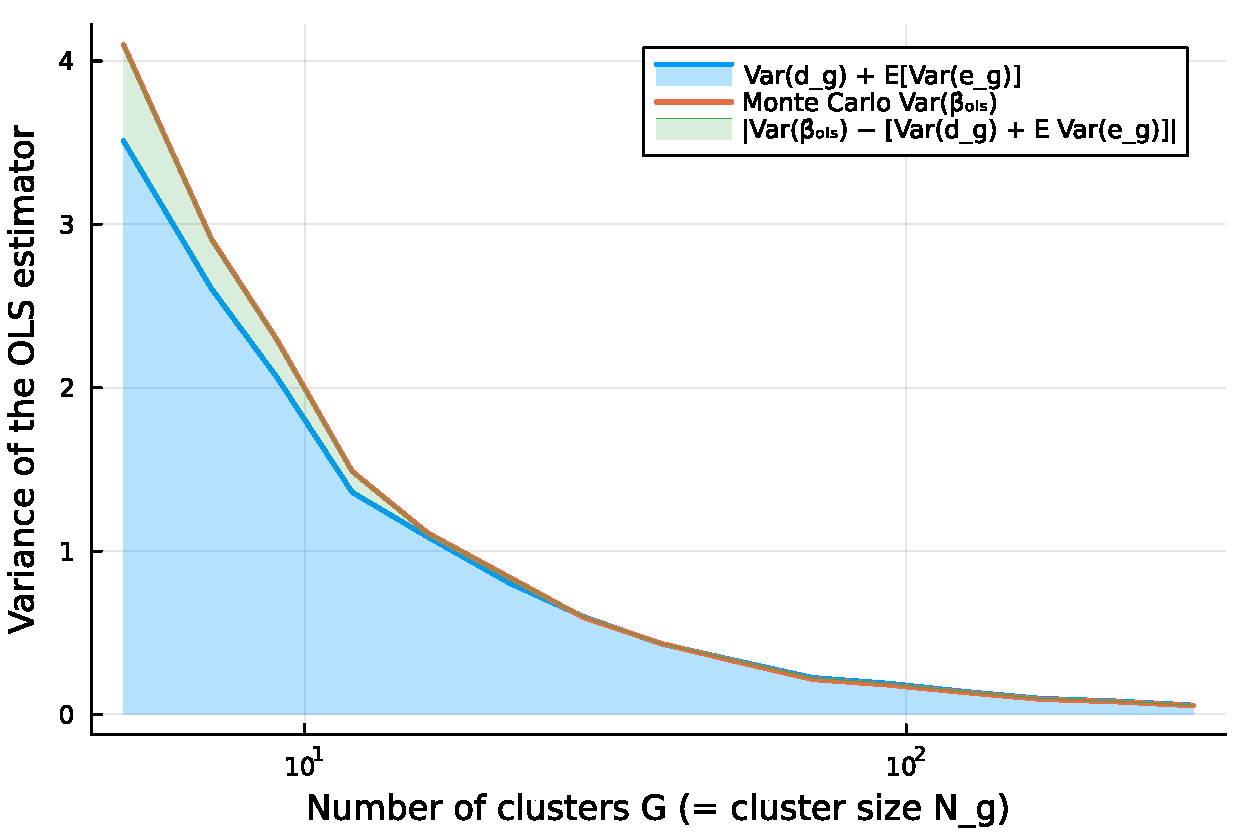
\includegraphics[width=1\linewidth,height=\textheight,keepaspectratio]{assets/decompositionOfBetaOLS.pdf}
\end{center}
\end{frame}

\begin{frame}{CRVE--White Differences as Heterogeneity Measure}
\phantomsection\label{crvewhite-differences-as-heterogeneity-measure}
\begin{itemize}
\tightlist
\item
  We test whether the \textbf{difference} between CRVE and White
  variance estimators\\
  captures the heterogeneity component \[
  \operatorname{Var}(\bar d_g),\quad
  d_g = \beta_g - \beta_{\text{APE}}.
  \]
\item
  For each design \((N_g, G)\):

  \begin{itemize}
  \tightlist
  \item
    compute average CRVE variance,
  \item
    compute average White variance,
  \item
    take their difference,
  \item
    compare it to \(\operatorname{Var}(\bar d_g)\) from the simulations.
  \end{itemize}
\end{itemize}
\end{frame}

\begin{frame}{Simulation-Based Comparison}
\phantomsection\label{simulation-based-comparison}
\begin{itemize}
\tightlist
\item
  For every \((N_g, G)\):

  \begin{itemize}
  \tightlist
  \item
    horizontal axis: \(\operatorname{Var}(\bar d_g)\) (variance of mean
    deviations),
  \item
    vertical axis: \[
    \mathbb{E}\big[\widehat{\operatorname{Var}}_{\text{CRVE}}\big]
    -
    \mathbb{E}\big[\widehat{\operatorname{Var}}_{\text{White}}\big].
    \]
  \end{itemize}
\item
  Each point is a design \((N_g,G)\):

  \begin{itemize}
  \tightlist
  \item
    color intensity encodes \(G\) (lighter = larger \(G\)).
  \end{itemize}
\item
  The 45-degree dashed line is the \textbf{benchmark} of perfect
  equality.
\end{itemize}
\end{frame}

\begin{frame}
\begin{center}
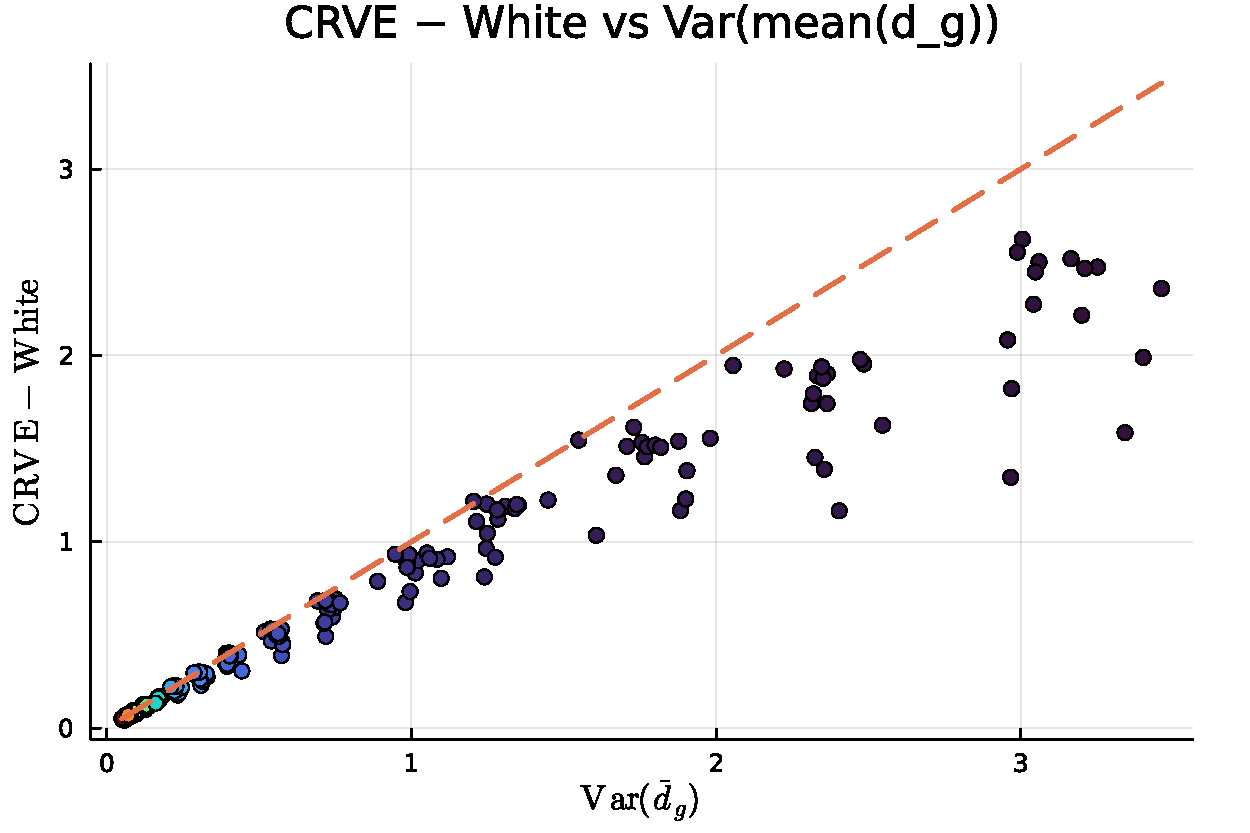
\includegraphics[width=1\linewidth,height=\textheight,keepaspectratio]{assets/dgEqualsDiff.pdf}
\end{center}
\end{frame}

\begin{frame}{Results and Interpretation}
\phantomsection\label{results-and-interpretation}
\begin{itemize}
\tightlist
\item
  Points lie very close to the 45-degree line:

  \begin{itemize}
  \tightlist
  \item
    CRVE--White differences almost exactly recover
    \(\operatorname{Var}(\bar d_g)\).
  \end{itemize}
\item
  Overall, the simulations support: \[
  \mathbb{E}\big[\widehat{\operatorname{Var}}_{\text{CRVE}}\big]
  -
  \mathbb{E}\big[\widehat{\operatorname{Var}}_{\text{White}}\big]
  \approx
  \operatorname{Var}(\bar d_g),
  \] and this relationship strengthens as the number of clusters \(G\)
  grows.
\end{itemize}
\end{frame}

\begin{frame}
\phantomsection\label{refs}
\begin{CSLReferences}{1}{0}
\bibitem[\citeproctext]{ref-imbens}
Abadie, Alberto, Susan Athey, Guido W. Imbens, and Jeffrey M.
Wooldridge. 2023. {``When Should You Adjust Standard Errors for
Clustering?''} \emph{The Quarterly Journal of Economics} 138 (1): 1--35.
\url{https://doi.org/10.1093/qje/qjac038}.

\bibitem[\citeproctext]{ref-cameron2015cluster}
Cameron, A. Colin, and Douglas L. Miller. 2015. {``A Practitioner's
Guide to Cluster-Robust Inference.''} \emph{Journal of Human Resources}
50 (2): 317--72. \url{https://doi.org/10.3368/jhr.50.2.317}.

\bibitem[\citeproctext]{ref-ibragimov2010t}
Ibragimov, Rustam, and Ulrich K Müller. 2010. {``T-Statistic Based
Correlation and Heterogeneity Robust Inference.''} \emph{Journal of
Business \& Economic Statistics} 28 (4): 453--68.

\bibitem[\citeproctext]{ref-wooldridge2003cluster}
Wooldridge, Jeffrey M. 2003. {``Cluster-Sample Methods in Applied
Econometrics.''} \emph{The American Economic Review} 93 (2): 133--38.
\url{http://www.jstor.org/stable/3132213}.

\end{CSLReferences}
\end{frame}




\end{document}
